%!TEX program = xelatex
\documentclass[10pt]{beamer}

\usetheme[progressbar=frametitle]{metropolis}
\usepackage{appendixnumberbeamer}

\usepackage{booktabs}
\usepackage[scale=2]{ccicons}

\usepackage{bm}
\usepackage{amsmath,amsfonts}
\newcommand{\Tr}{\operatorname{Tr}}

\usepackage{pgfplots}
\usepgfplotslibrary{dateplot}

\usepackage{xspace}
\newcommand{\themename}{\textbf{\textsc{metropolis}}\xspace}

\usepackage{graphicx}
\graphicspath{{../../../Figures/presentation_19_05/}}

\title{Statistical Properties of Geodesic Distances between Samples and Elementary Scatterers in PolSAR Imagery}
% \date{\today}
\date{}
\author{Danilo Fernandes, Alejandro C. Frery}
\institute{Laboratório de Computação Científica e Análise Numérica\\ Universidade Federal de Alagoas}
% \titlegraphic{\hfill\includegraphics[height=1.5cm]{logo.pdf}}

\begin{document}

\maketitle

\begin{frame}{Table of contents}
  \setbeamertemplate{section in toc}[sections numbered]
  \tableofcontents%[hideallsubsections]
\end{frame}

\section[Intro]{Introduction}

\begin{frame}[fragile]{Introduction}

    In Polarimetric SAR, a radar target is characterized by a scattering matrix $\bm S$ that describes the dependence of its scattering properties on the polarization. 
    It is defined as
    \[\mathbf{S} = 
    \begin{bmatrix}
    S_{\text{HH}} & S_{\text{HV}}\\
    S_{\text{VH}} & S_{\text{VV}}\\
    \end{bmatrix}
    ,\]
    
    where $\text{H}$ and $\text{V}$ denote, respectively, horizontal and vertical polarization.
  
\end{frame}

\begin{frame}[fragile]{Introduction}

    Another important matrix in PolSAR theory is the coherency $\bm{T}$ obtained by:
    $$
    \mathbf{T} = \frac{1}{L}\sum_{i=1}^{L}k_{p_i}k_{p_i}^{T*},
    $$
    where $k_p = 2^{-1/2} 
    \begin{bmatrix}
    S_{\text{HH}} + S_{\text{VV}} &S_{\text{HH}} - S_{\text{VV}} &2S_{\text{HV}}
    \end{bmatrix}^T
    $, $T$ denotes transposition,  $*$ denotes the complex conjugate, and $L$ is the number of looks.

\end{frame}

\begin{frame}[fragile]{Introduction}
  An approach to representing the PolSAR information in a real matrix is by the Kennaugh matrix. A Kennaugh matrix $\mathbf{K}$ can be obtained from the coherency matrix $\mathbf{T}$ in the following manner:
\[\mathbf{K} = 
\begin{bmatrix}
\frac{ T_{11} + T_{22} + T_{33} }{2} & \Re(T_{12}) & \Re(T_{13}) & \Im(T_{23})\\
\Re(T_{12}) & \frac{T_{11} + T_{22} - T_{33}}{2} & \Re(T_{23}) & \Im(T_{13})\\
\Re(T_{13}) & \Re(T_{23}) & \frac{ T_{11} - T_{22} + T_{33} }{2} & -\Im(T_{12})\\
\Im(T_{23}) & \Im(T_{13}) & -\Im(T_{12}) & \frac{ -T_{11} + T_{22} + T_{33} }{2}\\
\end{bmatrix}
.\]
\end{frame}

\begin{frame}[fragile]{Introduction}
    One way to measure the distance between two Kennaugh matrices $\bm K_1$ and $\bm K_2$ is through the Geodesic Distance, which is given by~\cite{ClassificationPolSARGeodesic}: 
    \begin{displaymath}
    \text{GD}(\mathbf{K_1}, \mathbf{K_2}) = \frac{2}{\pi} \cos^{-1} \left(\frac{\Tr(\mathbf{K_1}^T \mathbf{K_2})}{\sqrt{\Tr(\mathbf{K_1}^T \mathbf{K_1})} \sqrt{\Tr(\mathbf{K_2}^T \mathbf{K_2}})} \right),
    \end{displaymath}
    where $\Tr$ denotes the trace. It ranges between $[0,1]$. Consequently, the similarity can be defined as $f(K_1, K_2) = 1 - GD(K_1, K_2)$.
\end{frame}

\section[Histograms]{Histograms of similarities in relation to elementary targets}

\begin{frame}[fragile]{Histograms of similarities in relation to elementary targets}

\begin{figure}
    \centering
    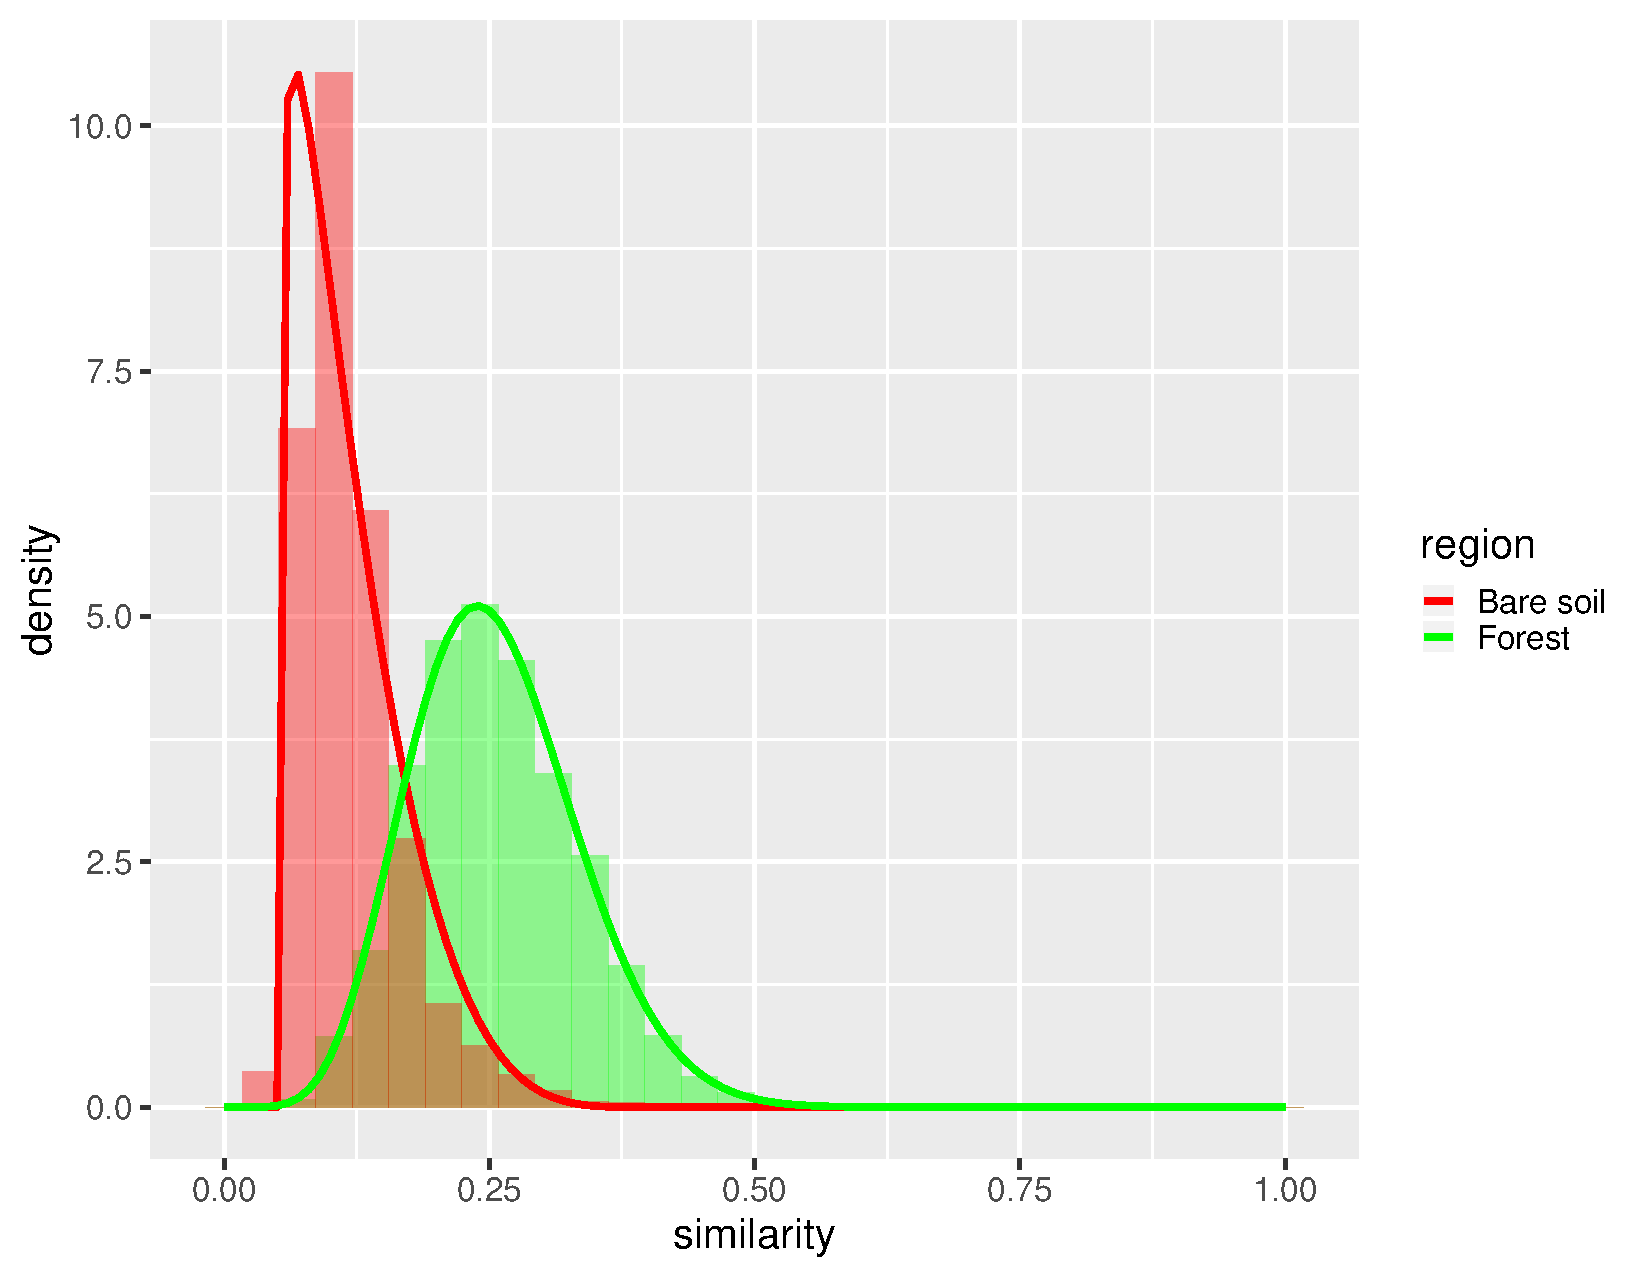
\includegraphics[width = .6\linewidth]{wvn.pdf}
    \caption{Similarity between PolSAR data from vegetation and bare soil regions in relation to the elementary target \textit{-1/4-wave}.}
    \label{fig:wvn}
\end{figure}
    
\end{frame}

\begin{frame}[fragile]{Histograms of similarities in relation to elementary targets}

\begin{figure}
    \centering
    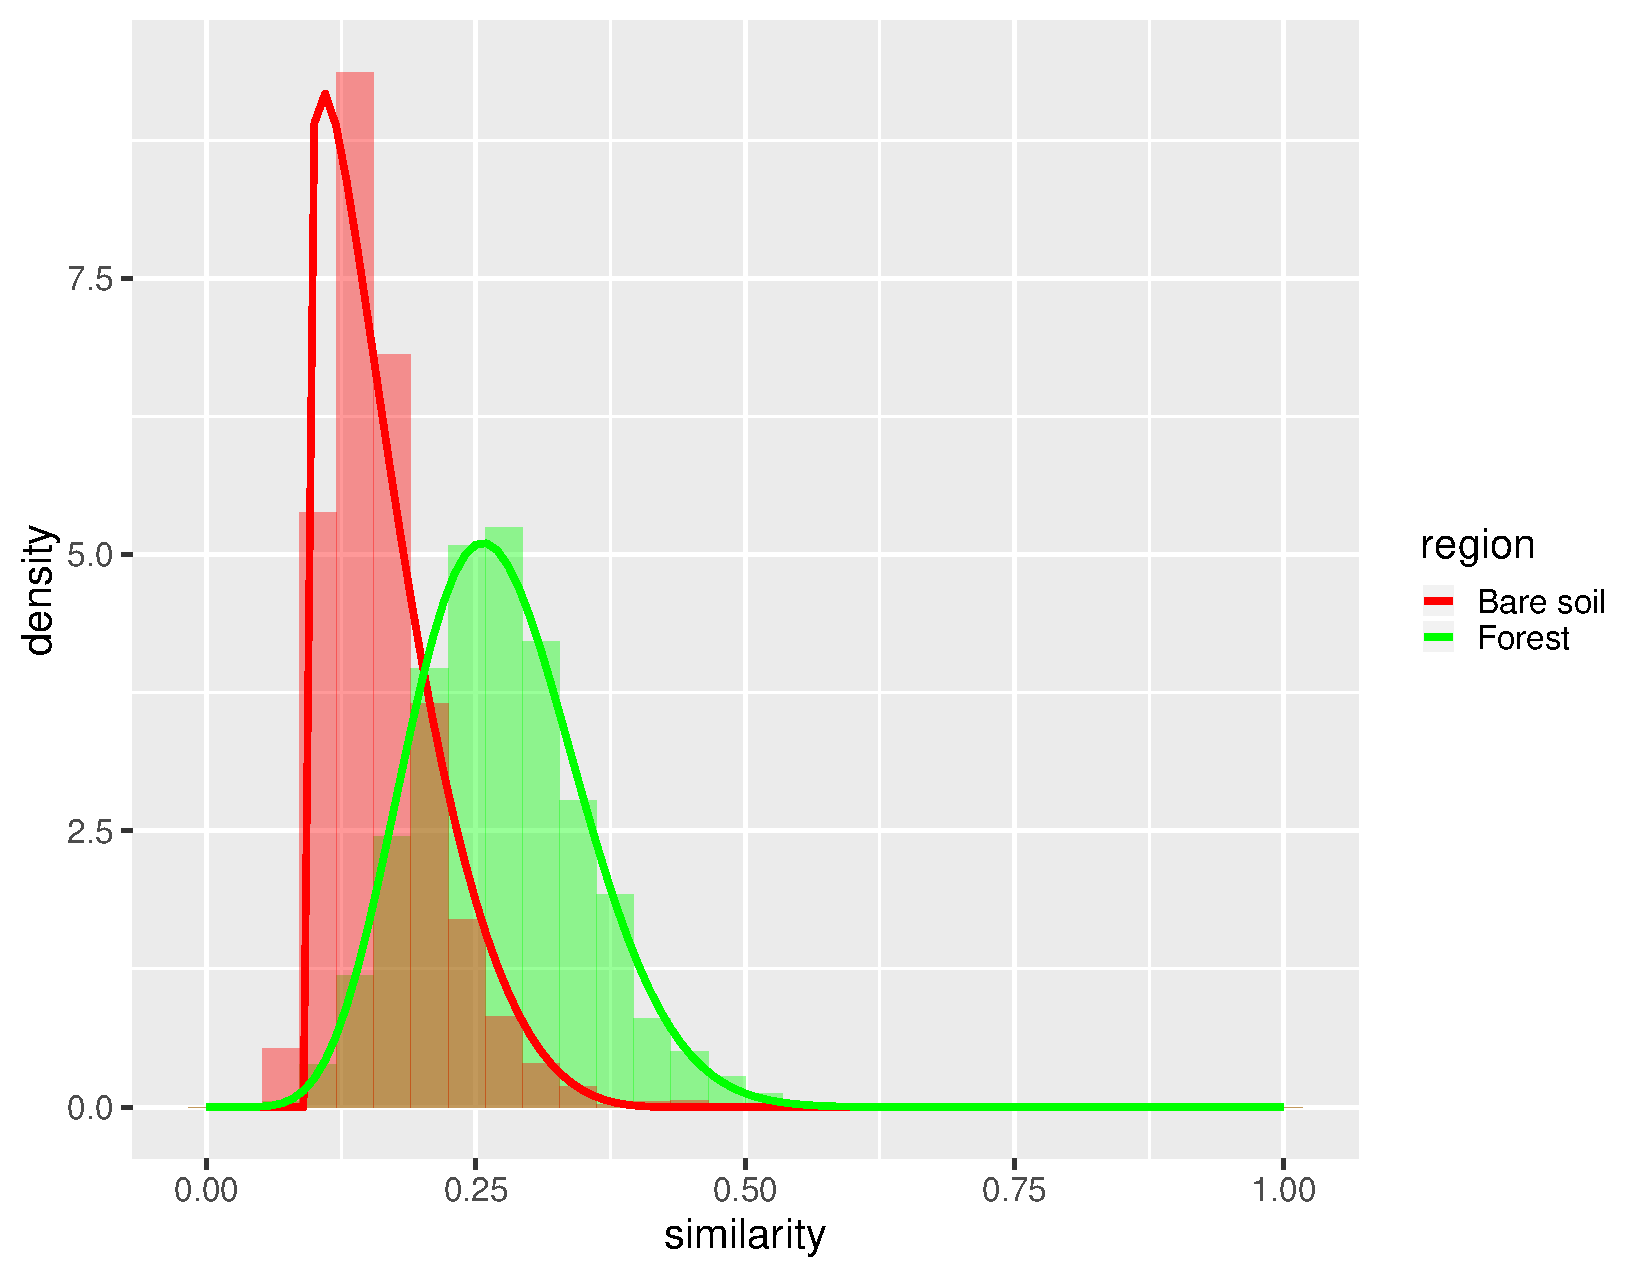
\includegraphics[width = .6\linewidth]{wvp.pdf}
    \caption{Similarity between PolSAR data from vegetation and bare soil regions in relation to the elementary target \textit{+1/4-wave}}
    \label{fig:wvp}
\end{figure}
    
\end{frame}

\begin{frame}[fragile]{Histograms of similarities in relation to elementary targets}

\begin{figure}
    \centering
    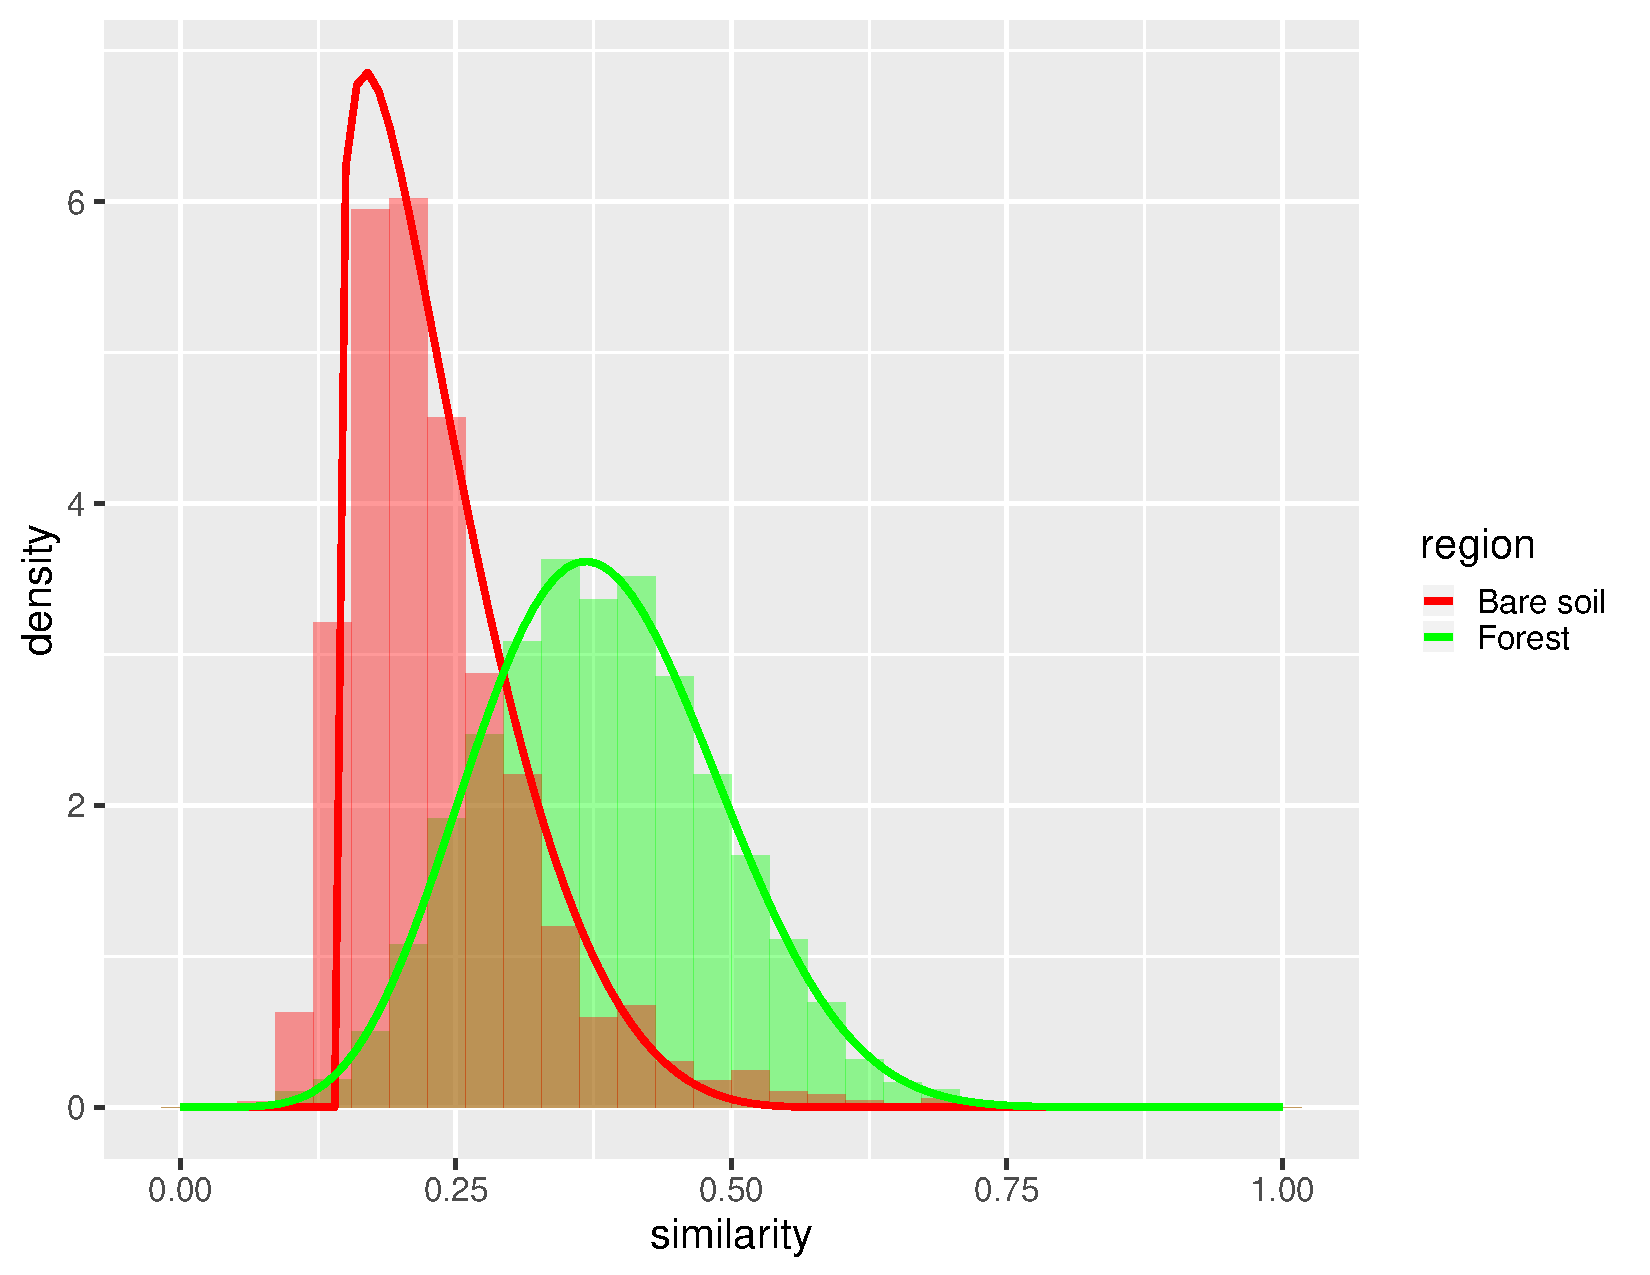
\includegraphics[width = .6\linewidth]{cy.pdf}
    \caption{Similarity between PolSAR data from vegetation and bare soil regions in relation to the elementary target \textit{cylinder}}
    \label{fig:cy}
\end{figure}
    
\end{frame}

\begin{frame}[fragile]{Histograms of similarities in relation to elementary targets}

\begin{figure}
    \centering
    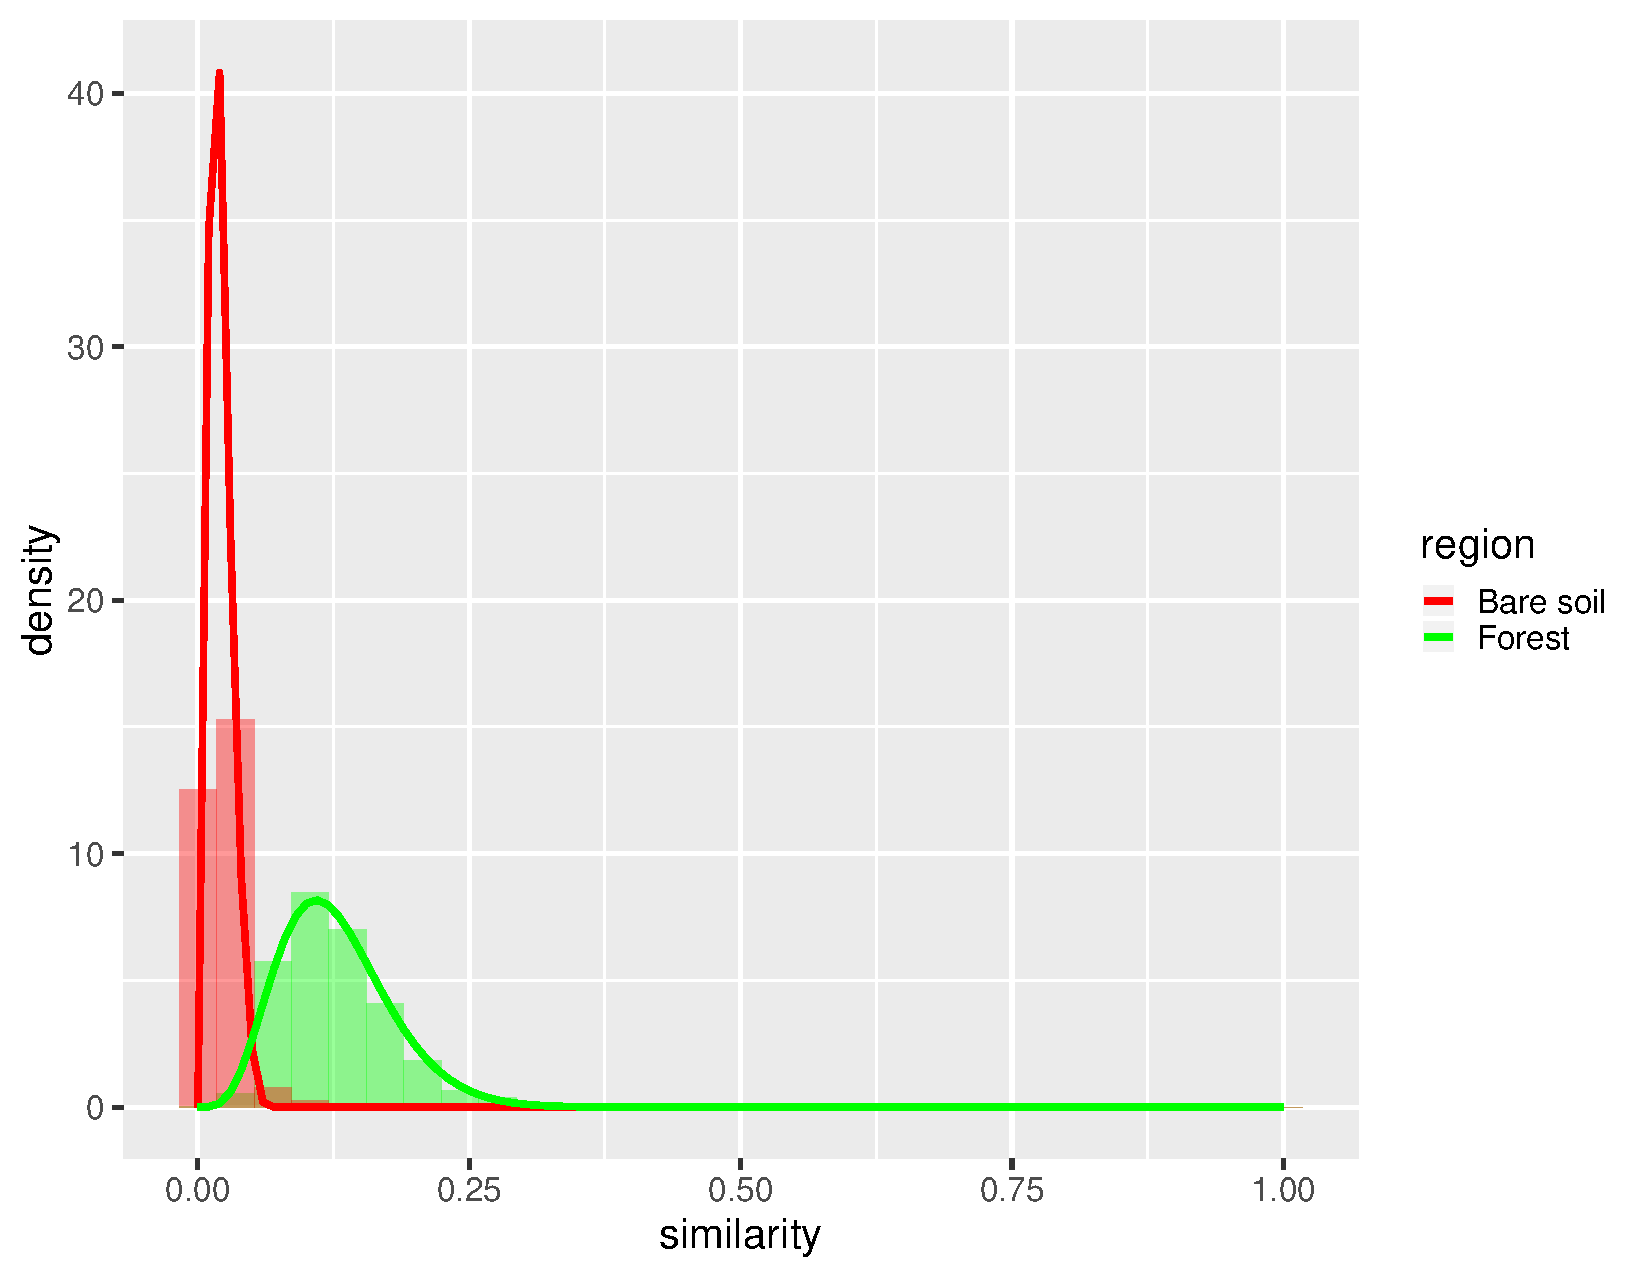
\includegraphics[width = .6\linewidth]{di.pdf}
    \caption{Similarity between PolSAR data from vegetation and bare soil regions in relation to the elementary target \textit{dihedral}}
    \label{fig:di}
\end{figure}
    
\end{frame}

\begin{frame}[fragile]{Histograms of similarities in relation to elementary targets}

\begin{figure}
    \centering
    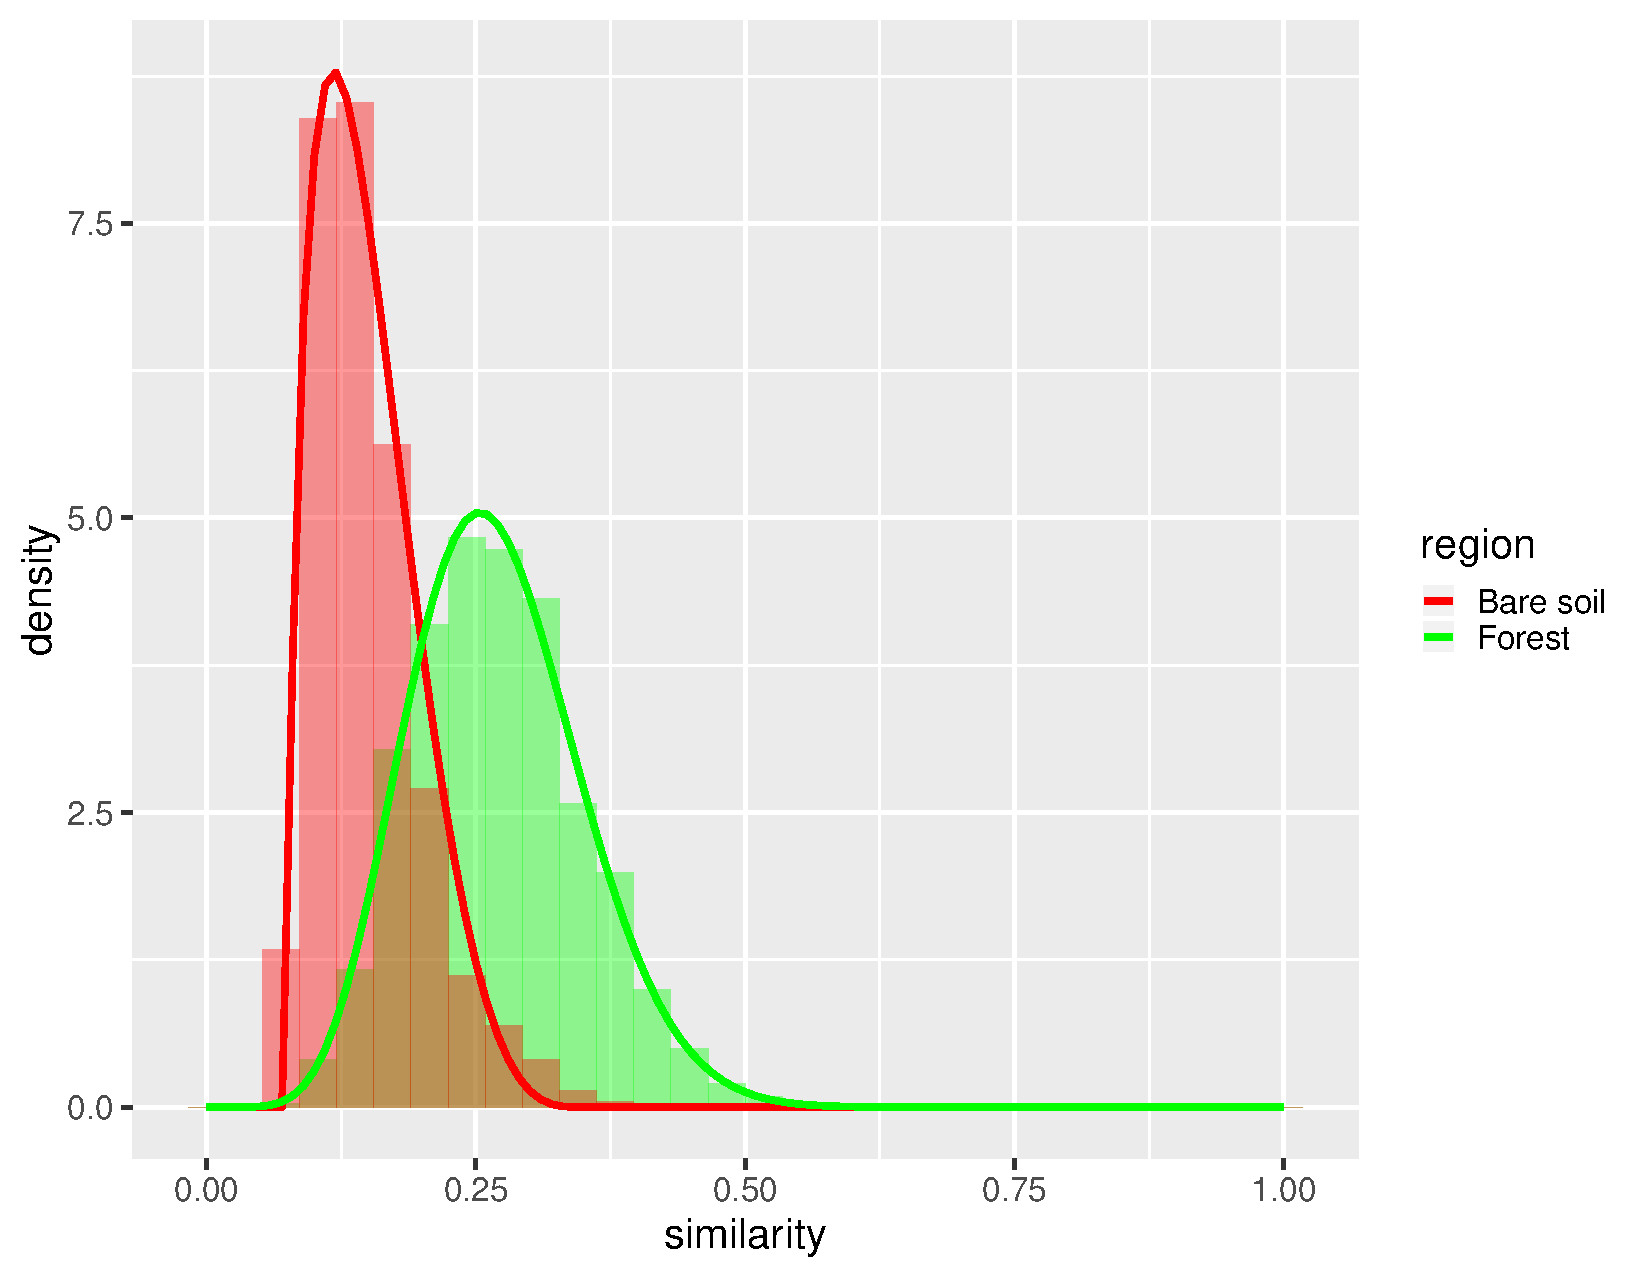
\includegraphics[width = .6\linewidth]{dip.pdf}
    \caption{Similarity between PolSAR data from vegetation and bare soil regions in relation to the elementary target \textit{dipole}}
    \label{fig:dip}
\end{figure}
    
\end{frame}

\begin{frame}[fragile]{Histograms of similarities in relation to elementary targets}

\begin{figure}
    \centering
    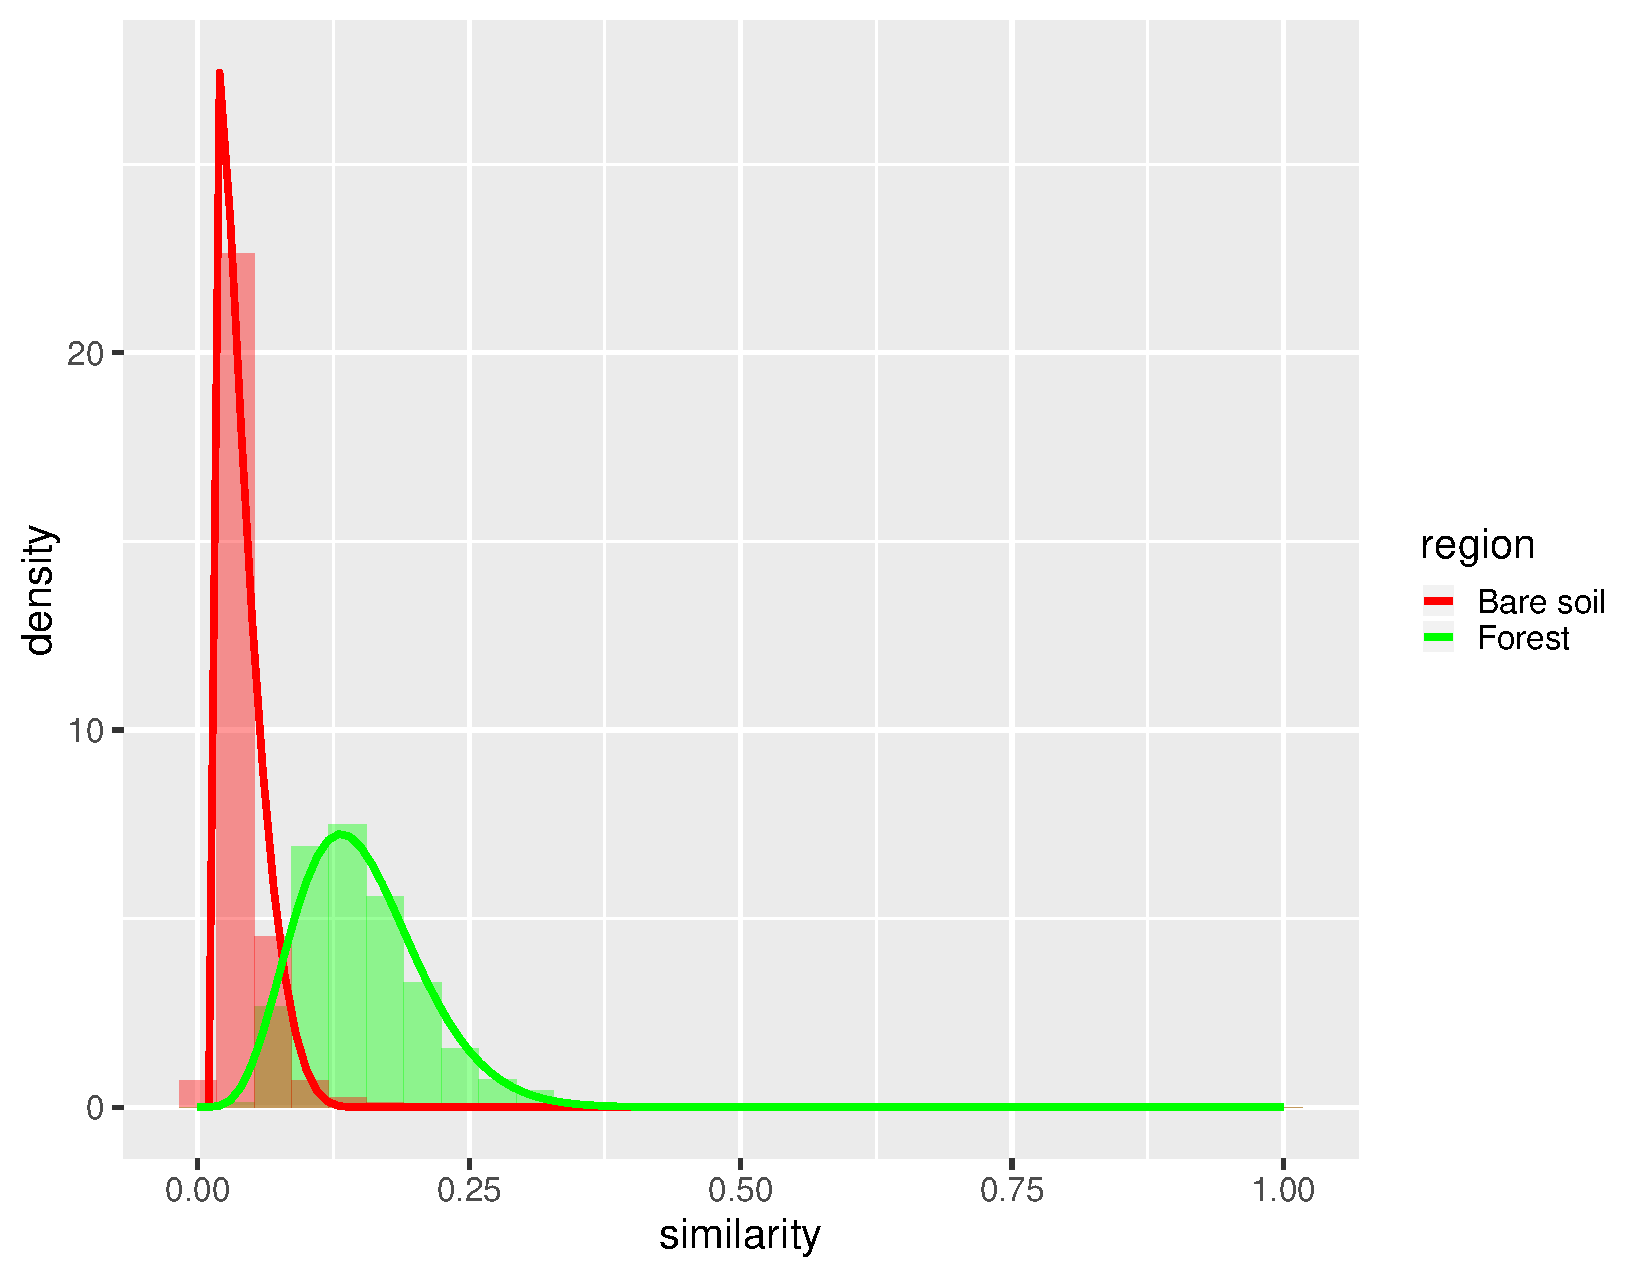
\includegraphics[width = .6\linewidth]{nd.pdf}
    \caption{Similarity between PolSAR data from vegetation and bare soil regions in relation to the elementary target \textit{narrow dihedral}}
    \label{fig:nd}
\end{figure}
    
\end{frame}

\begin{frame}[fragile]{Histograms of similarities in relation to elementary targets}

\begin{figure}
    \centering
    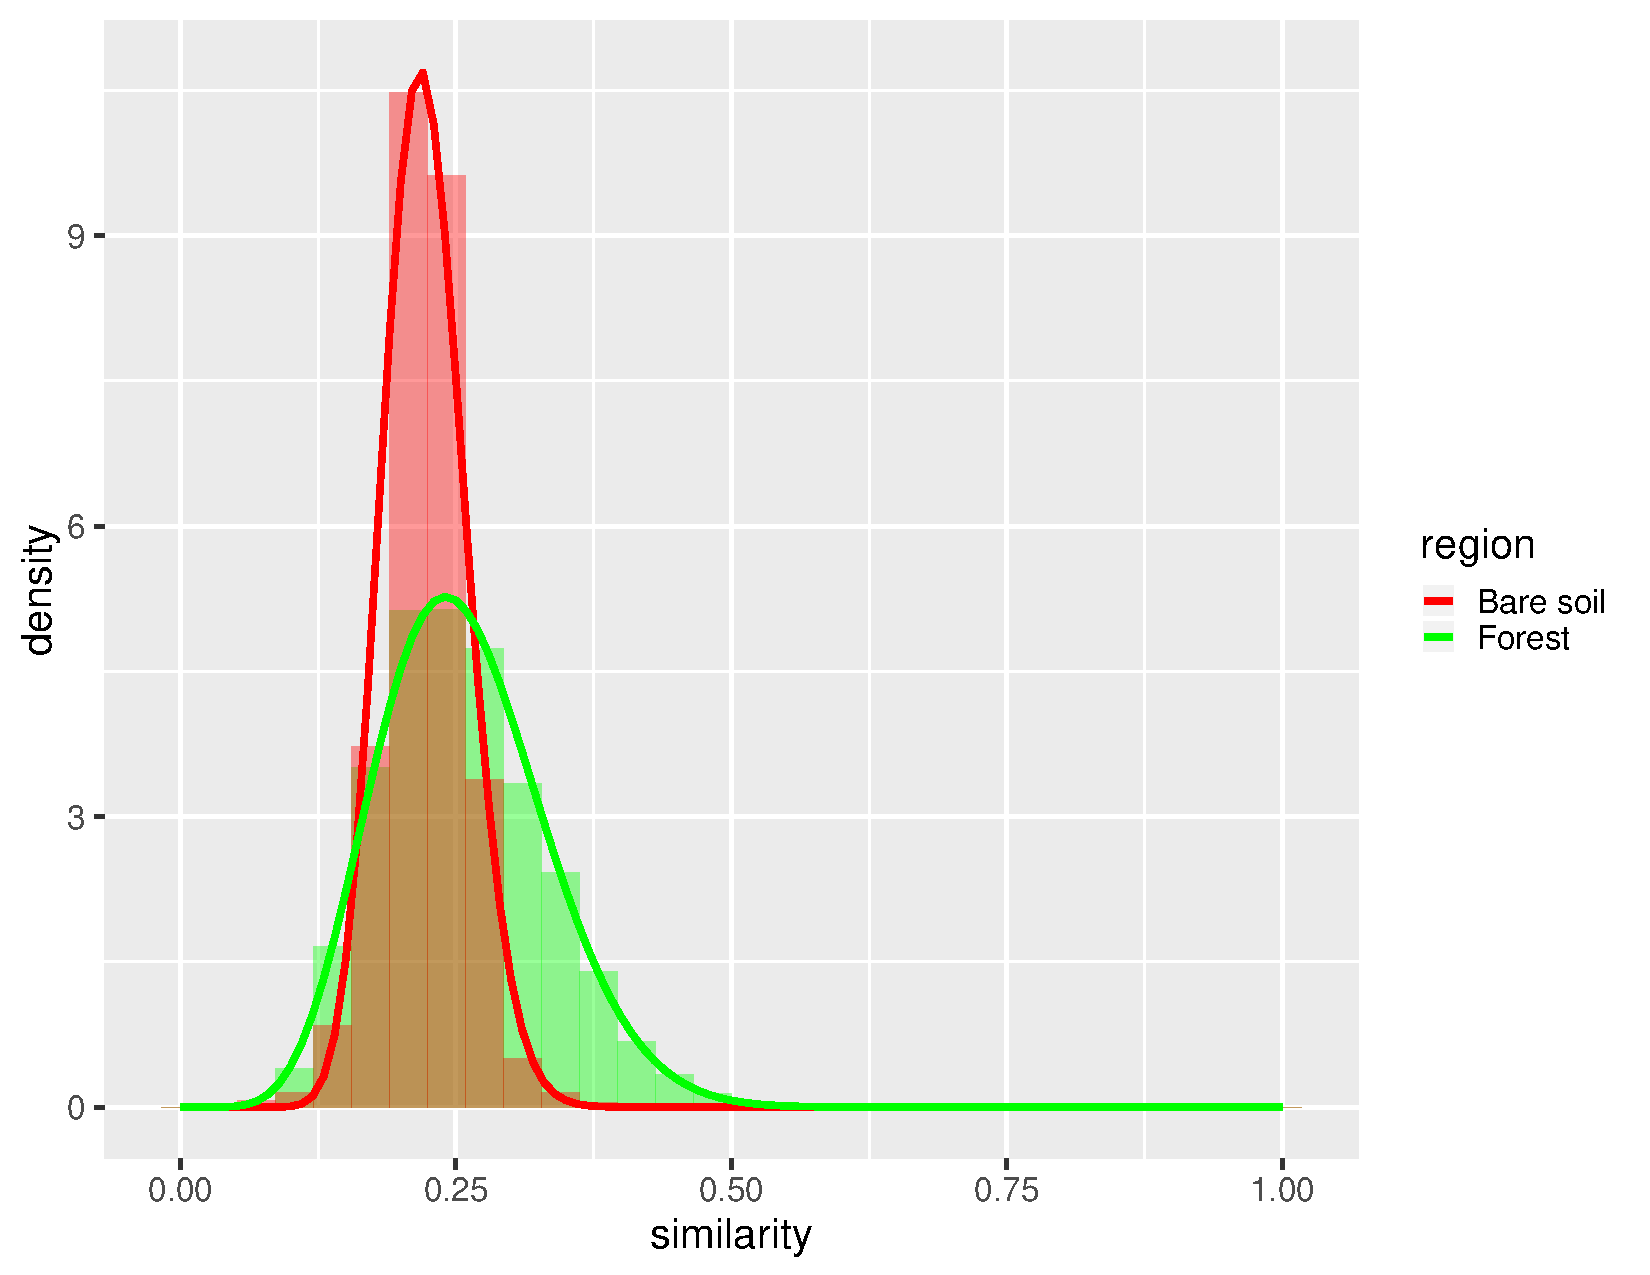
\includegraphics[width = .6\linewidth]{lh.pdf}
    \caption{Similarity between PolSAR data from vegetation and bare soil regions in relation to the elementary target \textit{left helix}}
    \label{fig:lh}
\end{figure}
    
\end{frame}

\begin{frame}[fragile]{Histograms of similarities in relation to elementary targets}

\begin{figure}
    \centering
    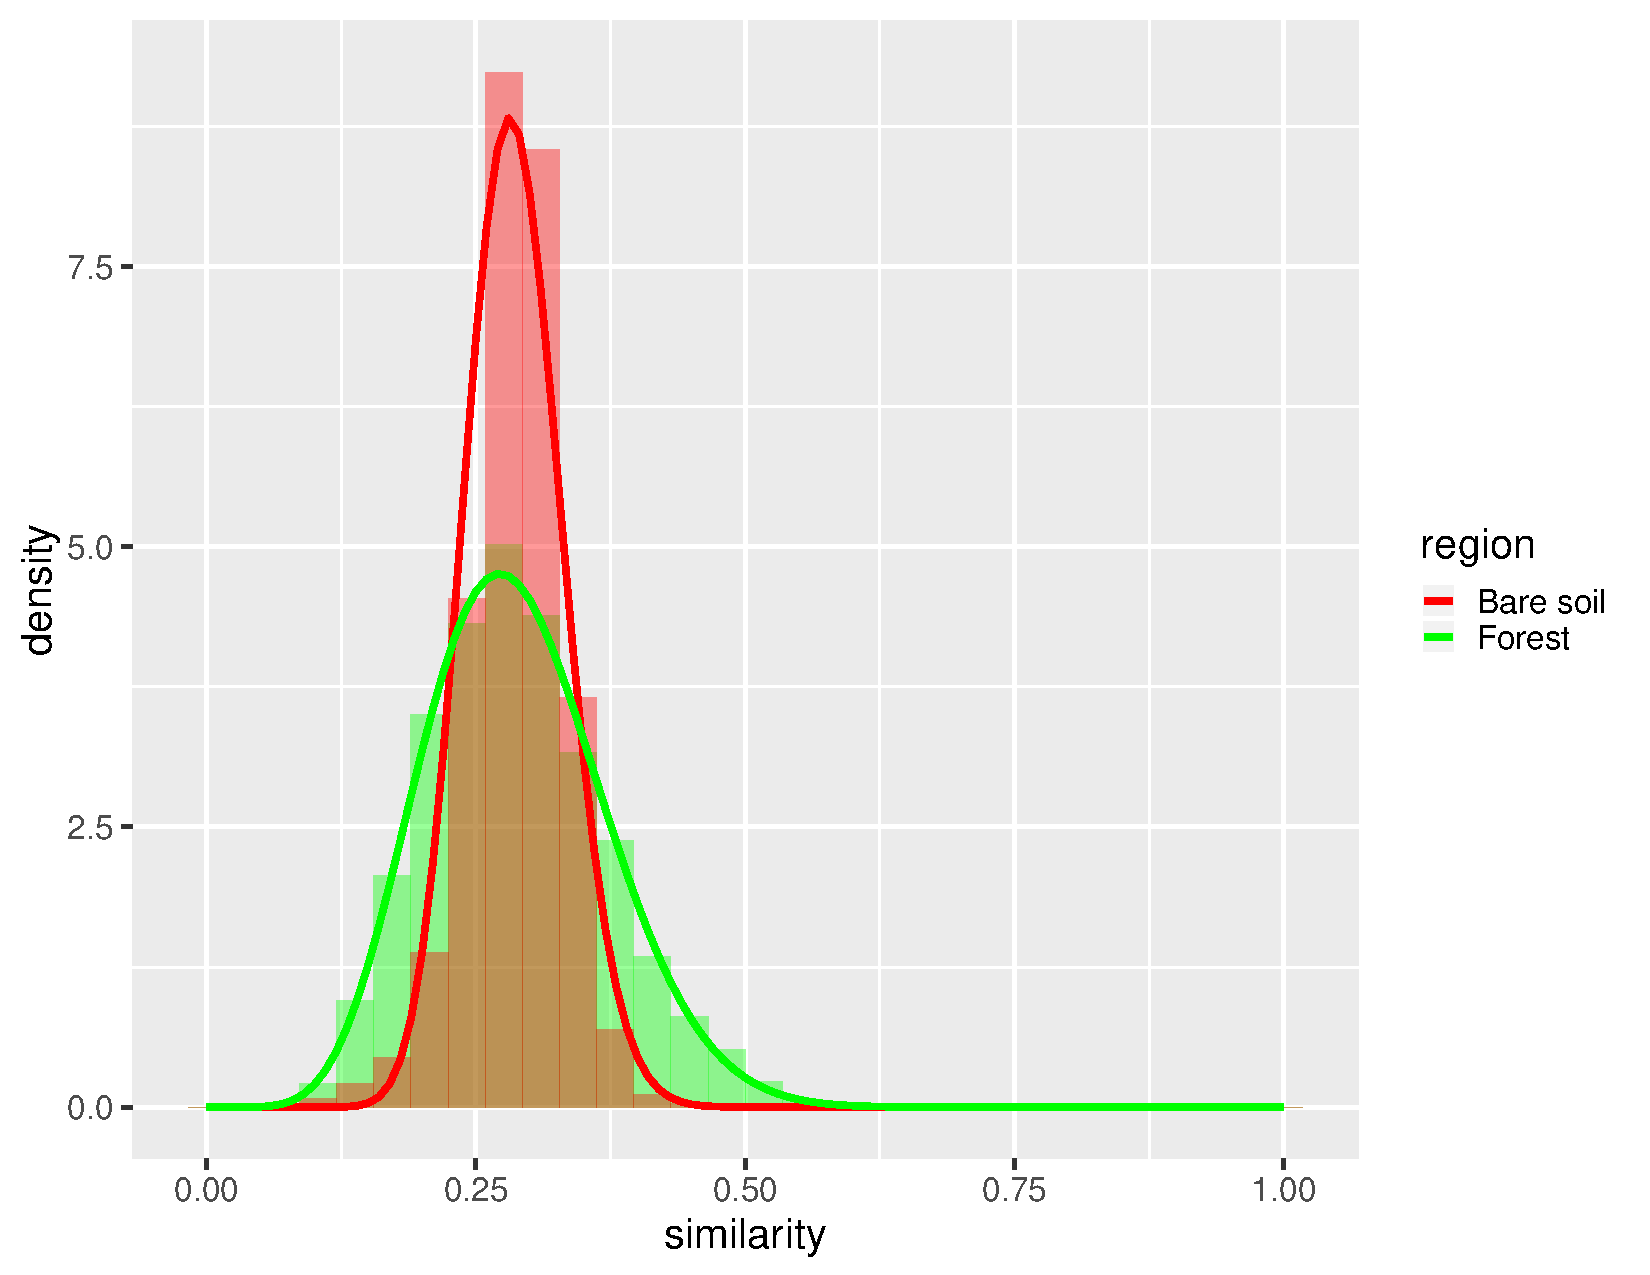
\includegraphics[width = .6\linewidth]{rh.pdf}
    \caption{Similarity between PolSAR data from vegetation and bare soil regions in relation to the elementary target \textit{right helix}}
    \label{fig:rh}
\end{figure}
    
\end{frame}

\begin{frame}[fragile]{Histograms of similarities in relation to elementary targets}

\begin{figure}
    \centering
    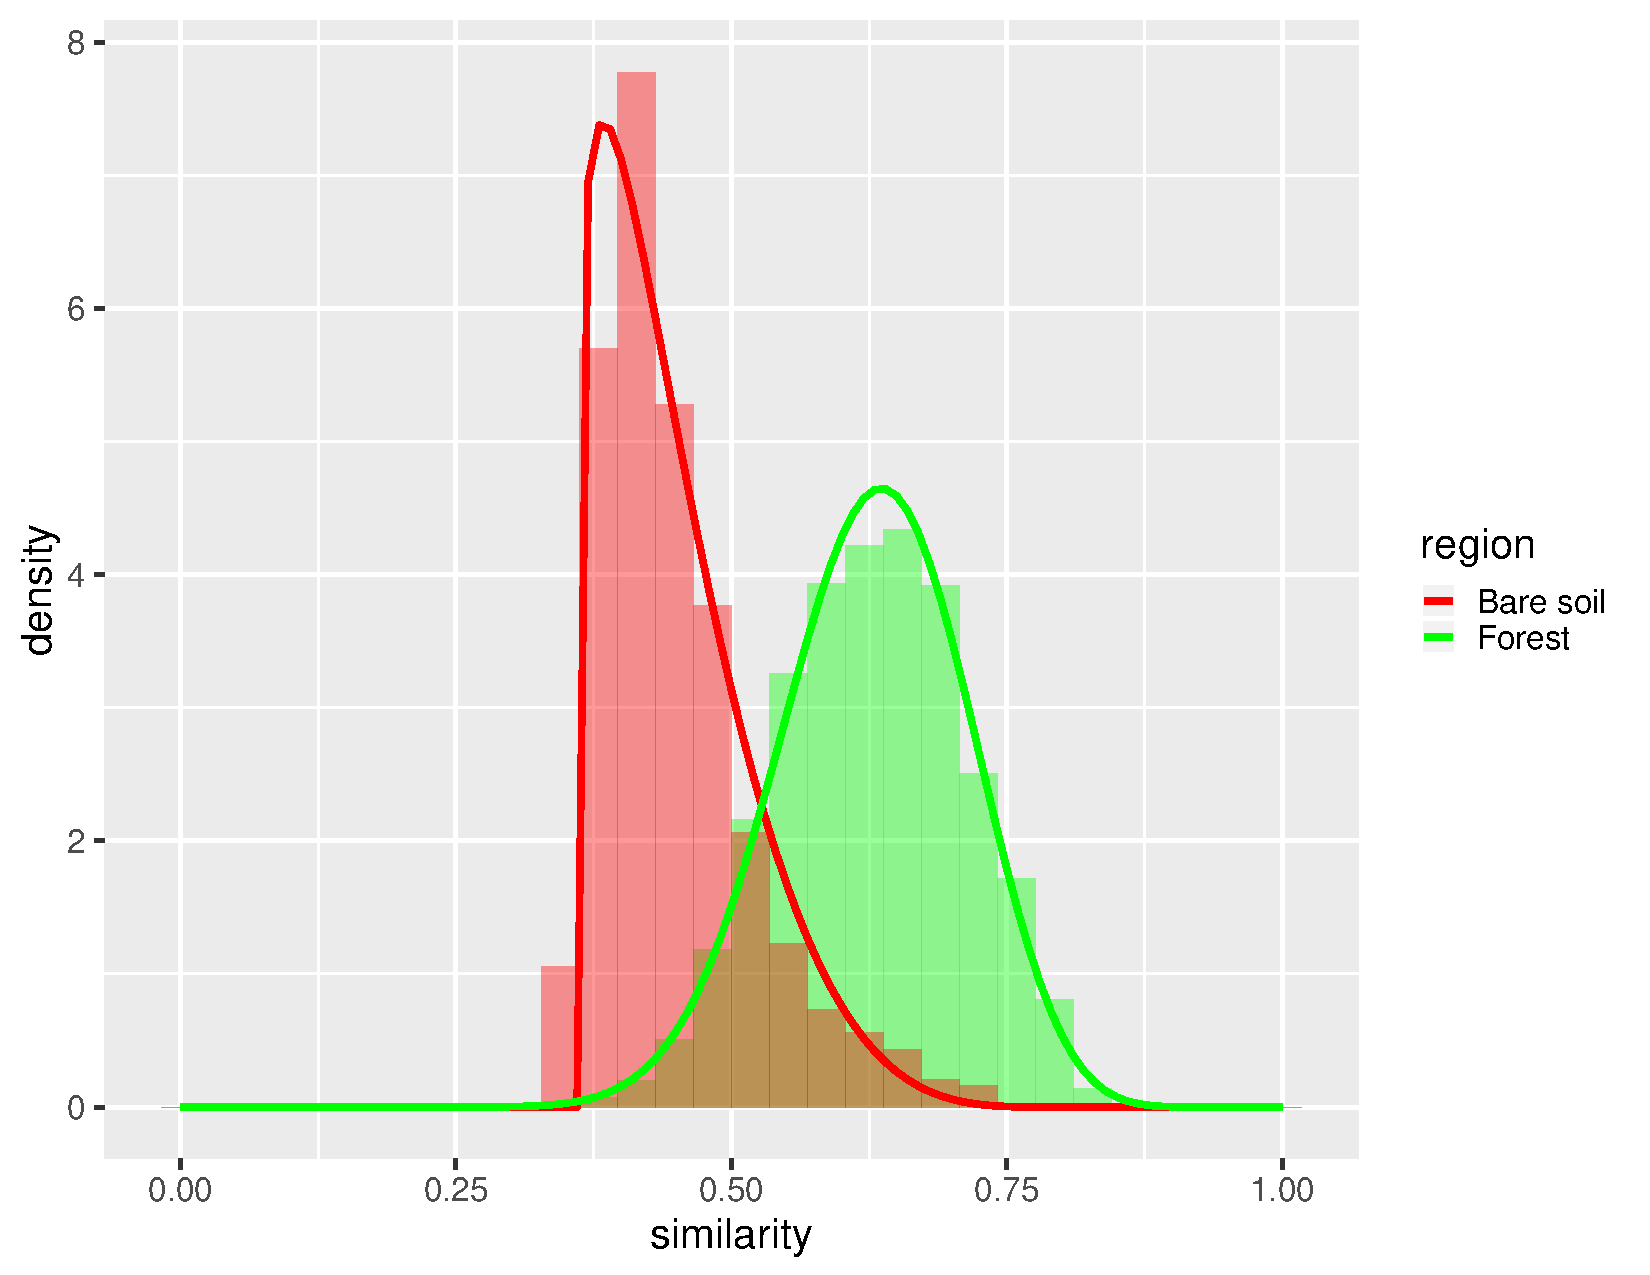
\includegraphics[width = .6\linewidth]{rv.pdf}
    \caption{Similarity between PolSAR data from vegetation and bare soil regions in relation to the elementary target \textit{random volume}}
    \label{fig:rv}
\end{figure}
    
\end{frame}

\begin{frame}[fragile]{Histograms of similarities in relation to elementary targets}

\begin{figure}
    \centering
    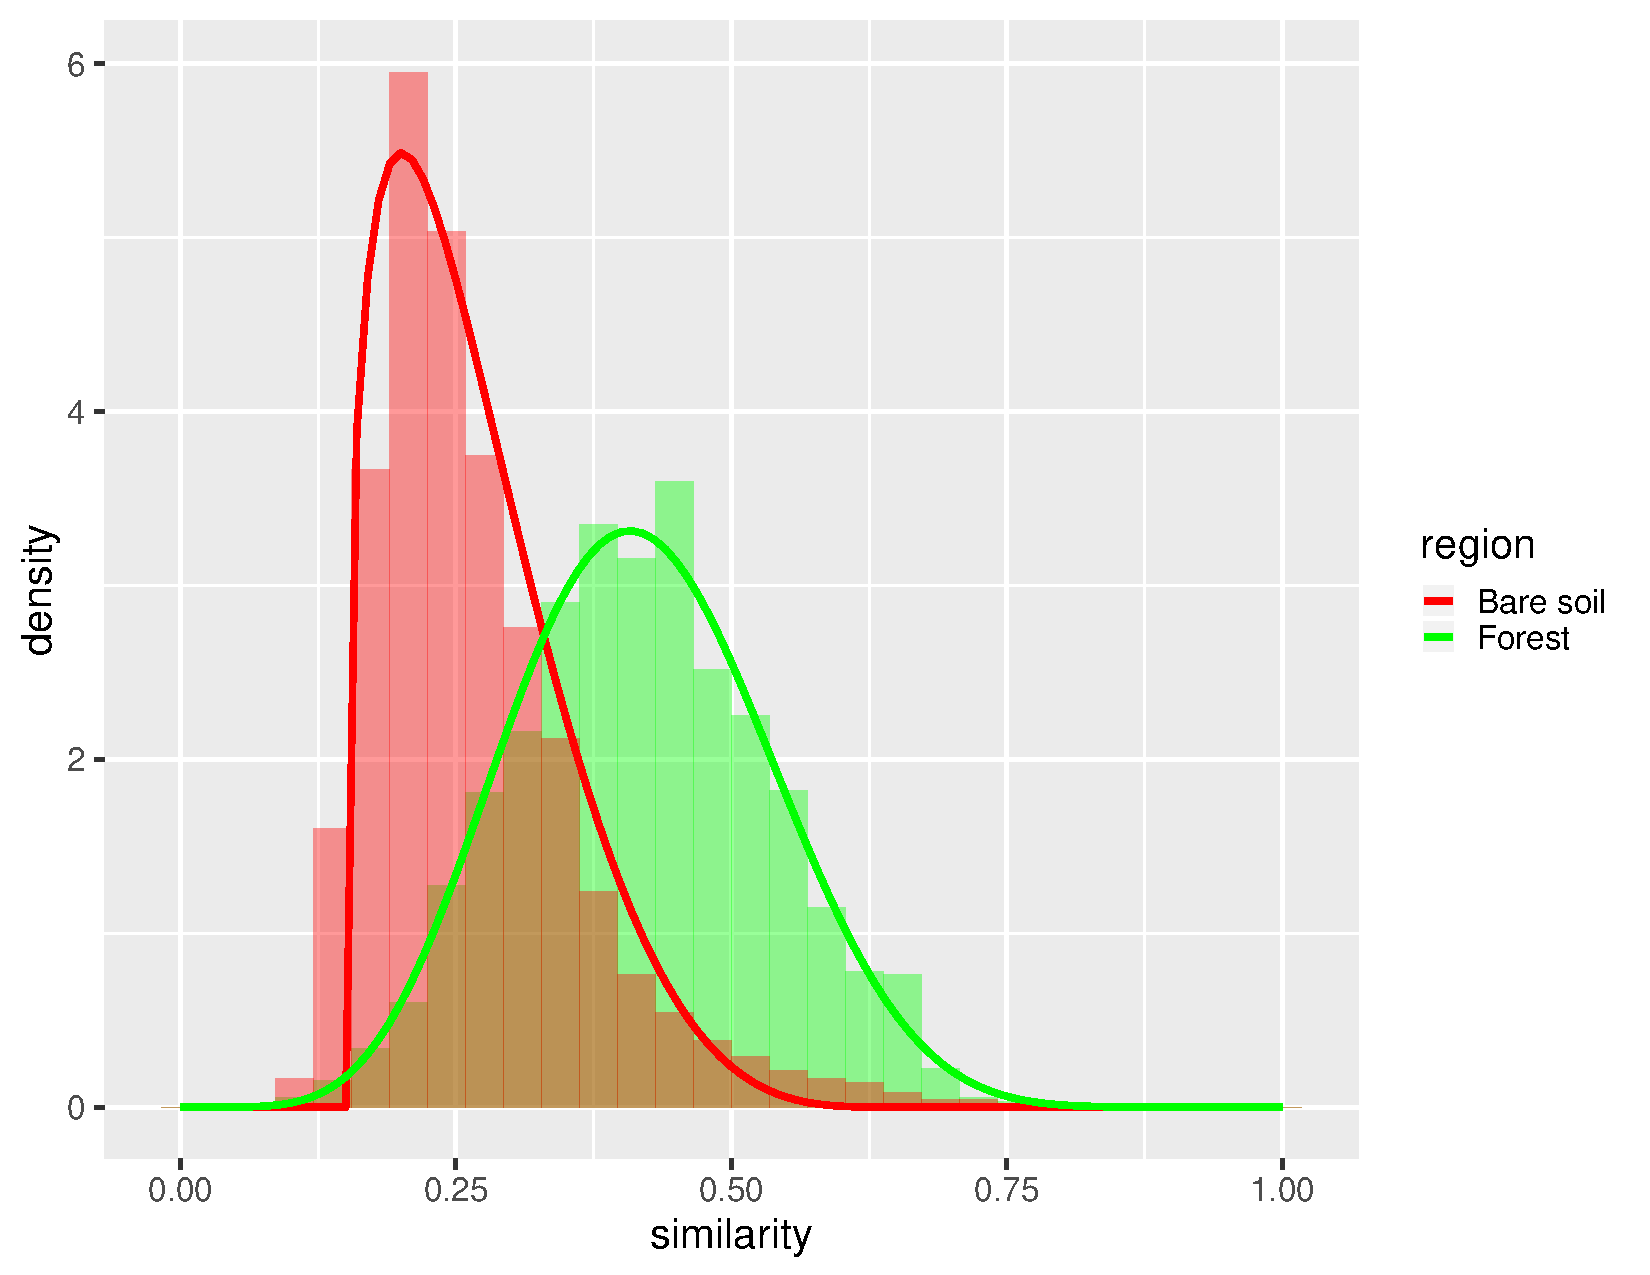
\includegraphics[width = .6\linewidth]{tr.pdf}
    \caption{Similarity between PolSAR data from vegetation and bare soil regions in relation to the elementary target \textit{trihedral}}
    \label{fig:tr}
\end{figure}
    
\end{frame}

\section[Estimation parameters]{Estimation of the parameters of the Beta distribution and mean for the analysed similarities}

\begin{frame}[fragile]{Estimation of the parameters of the Beta distribution and mean for the analysed similarities}
    \begin{table}[hbt]
    \centering
    %\caption{}\label{tab:estimated_params}     
    \begin{tabular}{lrrrrr}
    \toprule
    & $\min$ & $\max$ & $\widehat\alpha$ & $\widehat\beta$ & $\widehat\mu$\\ \midrule
    & \multicolumn{5}{c}{$-1/4$-wave}\\
    \cmidrule(lr){2-6}
    \textbf{Forest} & 0.000 & 1.000 & 7.830 & 22.758 & 0.255\\
    \textbf{Bare soil} & 0.055 & 0.400 & 1.127 & 4.872 & 0.119\\
    \midrule
    %
    & \multicolumn{5}{c}{$+1/4$-wave}\\
    \cmidrule(lr){2-6}
    \textbf{Forest} & 0.000 & 1.000 & 8.681 & 23.277 & 0.271\\
    \textbf{Bare soil} & 0.090 & 0.450 & 1.200 & 4.800 & 0.162\\
    \midrule
    %
    & \multicolumn{5}{c}{Cylinder}\\
    \cmidrule(lr){2-6}
    \textbf{Forest} & 0.000 & 1.000 & 7.500 & 12.165 & 0.381\\
    \textbf{Bare soil} & 0.140 & 0.600 & 1.243 & 4.756 & 0.235\\
    \bottomrule
    \end{tabular}
    \end{table}
\end{frame}

\begin{frame}[fragile]{Estimation of the parameters of the Beta distribution and mean for the analysed similarities}
    \begin{table}[hbt]
    \centering
    %\caption{}\label{tab:estimated_params}     
    \begin{tabular}{lrrrrr}
    \toprule
    & $\min$ & $\max$ & $\widehat\alpha$ & $\widehat\beta$ & $\widehat\mu$\\ \midrule
    & \multicolumn{5}{c}{Dihedral}\\
    \cmidrule(lr){2-6}
    \textbf{Forest} & 0.000 & 1.000 & 5.380 & 36.870 & 0.127\\
    \textbf{Bare soil} & 0.009 & 0.070 & 1.327 & 4.672 & 0.022\\
    \midrule
    %
    & \multicolumn{5}{c}{Dipole}\\
    \cmidrule(lr){2-6}
    \textbf{Forest} & 0.000 & 1.000 & 8.358 & 22.658 & 0.269\\
    \textbf{Bare soil} & 0.075 & 0.350 & 1.625 & 4.374 & 0.149\\
    \midrule
    %
    & \multicolumn{5}{c}{Narrow dihedral}\\
    \cmidrule(lr){2-6}
    \textbf{Forest} & 0.000 & 1.000 & 5.890 & 33.198 & 0.150\\
    \textbf{Bare soil} & 0.016 & 0.150 & 1.119 & 4.880 & 0.041\\
    \bottomrule
    \end{tabular}
    \end{table}
\end{frame}

\begin{frame}[fragile]{Estimation of the parameters of the Beta distribution and mean for the analysed similarities}
    \begin{table}[hbt]
    \centering
    %\caption{}\label{tab:estimated_params}     
    \begin{tabular}{lrrrrr}
    \toprule
    & $\min$ & $\max$ & $\widehat\alpha$ & $\widehat\beta$ & $\widehat\mu$\\ \midrule
    & \multicolumn{5}{c}{Left helix}\\
    \cmidrule(lr){2-6}
    \textbf{Forest} & 0.000 & 1.000 & 27.408 & 96.013 & 0.222\\
    \textbf{Bare soil} & 0.000 & 1.000 & 8.380 & 24.286 & 0.256\\
    \midrule
    & \multicolumn{5}{c}{Right helix}\\
    \cmidrule(lr){2-6}
    \textbf{Forest} & 0.000 & 1.000 & 28.522 & 71.238 & 0.285\\
    \textbf{Bare soil} & 0.000 & 1.000 & 8.316 & 20.574 & 0.287\\
    \midrule
    %
    & \multicolumn{5}{c}{Random volume}\\
    \cmidrule(lr){2-6}
    \textbf{Forest} & 0.000 & 1.000 & 20.074 & 11.910 & \textcolor{red}{0.627}\\
    \textbf{Bare soil} & 0.360 & 0.800 & 1.218 & 4.781 & \textcolor{red}{0.449}\\
    \bottomrule
    \end{tabular}
    \end{table}
\end{frame}

\begin{frame}[fragile]{Estimation of the parameters of the Beta distribution and mean for the analysed similarities}
    \begin{table}[hbt]
    \centering
    %\caption{}\label{tab:estimated_params}     
    \begin{tabular}{lrrrrr}
    \toprule
    & $\min$ & $\max$ & $\widehat\alpha$ & $\widehat\beta$ & $\widehat\mu$\\ \midrule
    & \multicolumn{5}{c}{Trihedral}\\
    \cmidrule(lr){2-6}
    \textbf{Forest} & 0.000 & 1.000 & 7.197 & 9.996 & 0.418\\
    \textbf{Bare soil} & 0.150 & 0.650 & 1.408 & 4.592 & 0.267\\
    \bottomrule
    \end{tabular}
    \end{table}
\end{frame}

\section[Goodness-of-fit test]{p-values obtained by Kolmogorov-Smirnov goodness-of-fit test}

\begin{frame}{p-values obtained by Kolmogorov-Smirnov goodness-of-fit test}
    \begin{table}[hbt]
    \centering
    %\caption{$p$-values of the Kolmogorov-Smirnov goodness-of-fit test of the similarity w.r.t. elementary backscatterers}\label{tab:pvalues_table}
    \begin{tabular}{lrrrrr}
    \toprule
    & $-1/4$- & $+1/4$- & Cylinder & Dihedral & Dipole\\
    & wave & wave & & &\\
    \cmidrule(lr){2-6}
    \textbf{Forest} & 0.979 & 0.808 & 0.763 & 0.733 & 0.975\\
    \textbf{Bare soil} & 0.361 & 0.893 & 0.264 & 0.443 & 0.475\\
    \midrule
    & Left & Narrow & Random & Right & Trihedral\\
    & helix & dihedral & volume & helix & \\
    \cmidrule(lr){2-6}
    \textbf{Forest} & 0.959 & 0.787 & 0.589 & 0.344 & 0.582\\
    \textbf{Bare soil} & 0.099 & 0.206 & 0.480 & 0.072 & 0.127\\
    \bottomrule
    \end{tabular} 
    \end{table}
\end{frame}

\begin{frame}[allowframebreaks]{References}

  \bibliography{../../../Bibliography/references}
  \bibliographystyle{abbrv}

\end{frame}

\end{document}
